\section{Островные ЭА.}
Общая идея
\begin{itemize}
    \item Несколько эволюционных алгоритмов («островов»), работающих независимо и иногда обменивающихся особями
\end{itemize}  
Островные алгоритмы приводят к повышению разнообразия
\begin{itemize}
    \item Одна особь не может «завоевать» всю популяцию сразу: сначала ей придется пережить миграции
    \item Разные острова могут фокусироваться на разных локальных оптимумах 
 
        Те можем искусственно разбить пространство поиска на части, и каждый остров будет искать оптимум в своем подпространстве. Когда каждый остров найдет свой оптимум, мы можем запустить новый алгоритм оптимизации, где исходной популяцией будут результаты работы прошлого алгоритма. Тогда оптимум, найденный новым алгоритмом будет претендовать на глобальность.
\end{itemize} 
Островные алгоритмы как распределенные вычисления.
\begin{itemize}
    \item Эволюция каждого острова производится на отдельном ядре/ноде. Остров или однопоточный, или с общей памятью. Миграция = передача сообщений, существенно меньшие потоки данных
\end{itemize}


Промежуток времени между миграциями называется эпохой. Период эпохи и принцип селекции мигрантов являются настраивыми параметрами алгоритма.

\subsection*{Топологии островных алгоритмов}

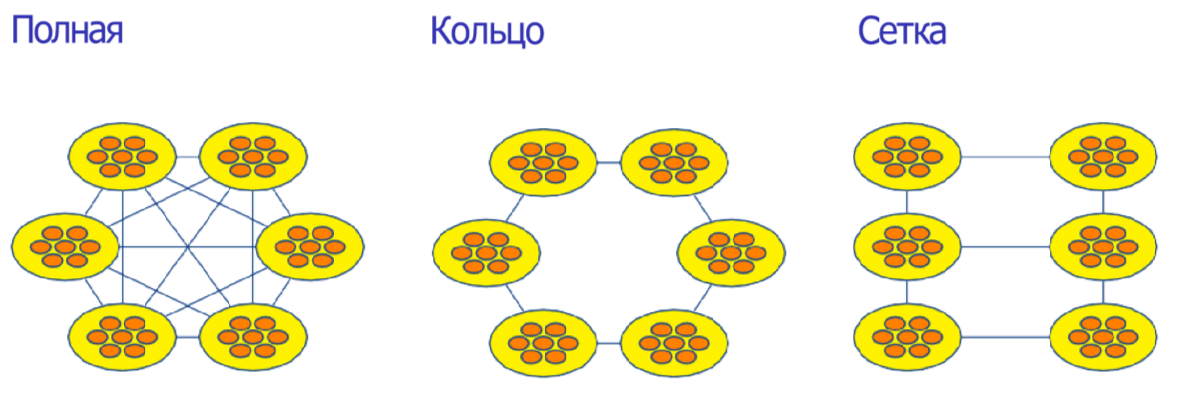
\includegraphics[width=14cm]{images/67_topology.png} 

\textit{На самом деле ноды соединены не одним каналом, как на картинке, а двумя. Один нужен для передачи особи, а другой - для передачи синхронизирующих сообщений.
}


Вариативность путей миграции влияет на эффективность алгоритма. Так как разные топологии открывают разные возможные пути миграций, выбор топологии - один из важнейших параметров алгоритма.

Чем сложнее связи, тем сложнее отследить путь миграции особи

\subsection*{Алгоритмы миграции в островных алгоритмах}

\textbf{Выбор особей для миграции}:
Мигрируют либо лучшие особи, либо случайные особи. Как правило за раз из 1 острова выбирается 1 особь для миграции. 

Не редкой является ситуация, когда на одном острове получились особи сильно лучше, чем на других. Тогда при стратегиях выбора мигрантов, описанных выше, происходит вырождение. \textbf{Чтобы бороться с такой ситуацией мигрируют самые деградировавшие особи}. Лучше на всех островах будет 15\% деградирадировавших особей, чем на одном 100\%. Ведь если на одном острове все особи будут деградировавшими, он перестанет быть полезным и "выпадет" из алгоритма. 

Это не было сказано явно, но я вижу еще другой вариант вырожждения: если один остров станет лучше других, особи именно с этого острова будут мигрировать в другие почти всегда. В итоге мы потеряем разнообразие, в следствие чего островной алгоритм становится не лучше обычного генетического алгоритма 

\textbf{Частота миграции}: раз в итерацию / раз в n итераций / при обновлении лучшей особи

\textbf{Куда мигрируем?}: либо к случайному соседу (за исключением соседа, к которому мигрировали на предыдущем шаге), либо во все соседние острова.

\textbf{Условие принятия мигранта}:
\begin{itemize}
    \item Безусловно принимаем, удаляем худшую особь из своих
    \item Принимаем, только если не лучше нашей лучшей особи 
\end{itemize}
